% !TeX TXS-program:compile = txs:///pdflatex/[--shell-escape]
% Le truc au-dessus pour avoir l'option shell-escape qui permet de faire du minted.
\documentclass[12pt]{article}

% Affichage ou non des reponses aux questions & exercices
\newif\ifDispRep
%\DispReptrue  % Show the text
\DispRepfalse % Hide the text

% Version du document
\newcommand{\versiondoc}{v0.1}

% Incorporation tous éléments de préambule communs à tous mes cours
% Sans chemin relatif parce que TexStudio lancé depuis un script qui prend en compte la variable d'environnement TEXINPUTS
\usepackage{CoursLFC}

% Eléments de l'en-tête et de la page de garde spécifiques à ce doc
\newcommand{\classe}{1\textsuperscript{ère} NSI}
\newcommand{\themecours}{Architecture Système}
\newcommand{\datedoc}{mai 2024}

% Page de garde mise en page
\title
	{\vspace{2cm}
		{\Large
		\textit
			{
				\classe\hspace{0.1cm}
				\textemdash\
				\hspace{0.1cm}
				\themecours
			}
			
		\vspace{1cm}
		\huge{TP Shell UNIX}
		
		\large{\textit{tiré d'un TP de Charles Poulmaire}}
		
}
		 
		\vspace{1cm}
	}
\author{\etablissement}
\date{
	\auteur,
	\datedoc,
	\footnotesize{\textit{\versiondoc}} 
	\vspace{3cm}
	}

% Header & Footer
\lfoot{\etabshort}
\cfoot{\thepage}
\rfoot{\classe, \anneescol}
\renewcommand{\footrulewidth}{0.2pt}
\lhead{}
\chead{}
\rhead{}
\renewcommand{\headrulewidth}{0pt}

\begin{document}
	
	\maketitle
	% pas de footer sur la première page
	\thispagestyle{empty}
	\vspace{\baselineskip}
	
	\pagebreak
	
	
	\textbf{Tout ce qui est décrit dans ce document va être à réaliser dans le terminal de votre machine HP NSI, que vous pouvez lancer depuis la barre de tâches (le logo est un carré noir avec un ">" blanc dessus).}
	
	\section{Arborescence de fichiers}
	
	L'arborescence de fichiers représente l'organisation des dossiers et fichiers dans votre ordinateur. Voici un exemple d’une arborescence extrêmement basique:
	
	\begin{figure}[H]
		\centering
		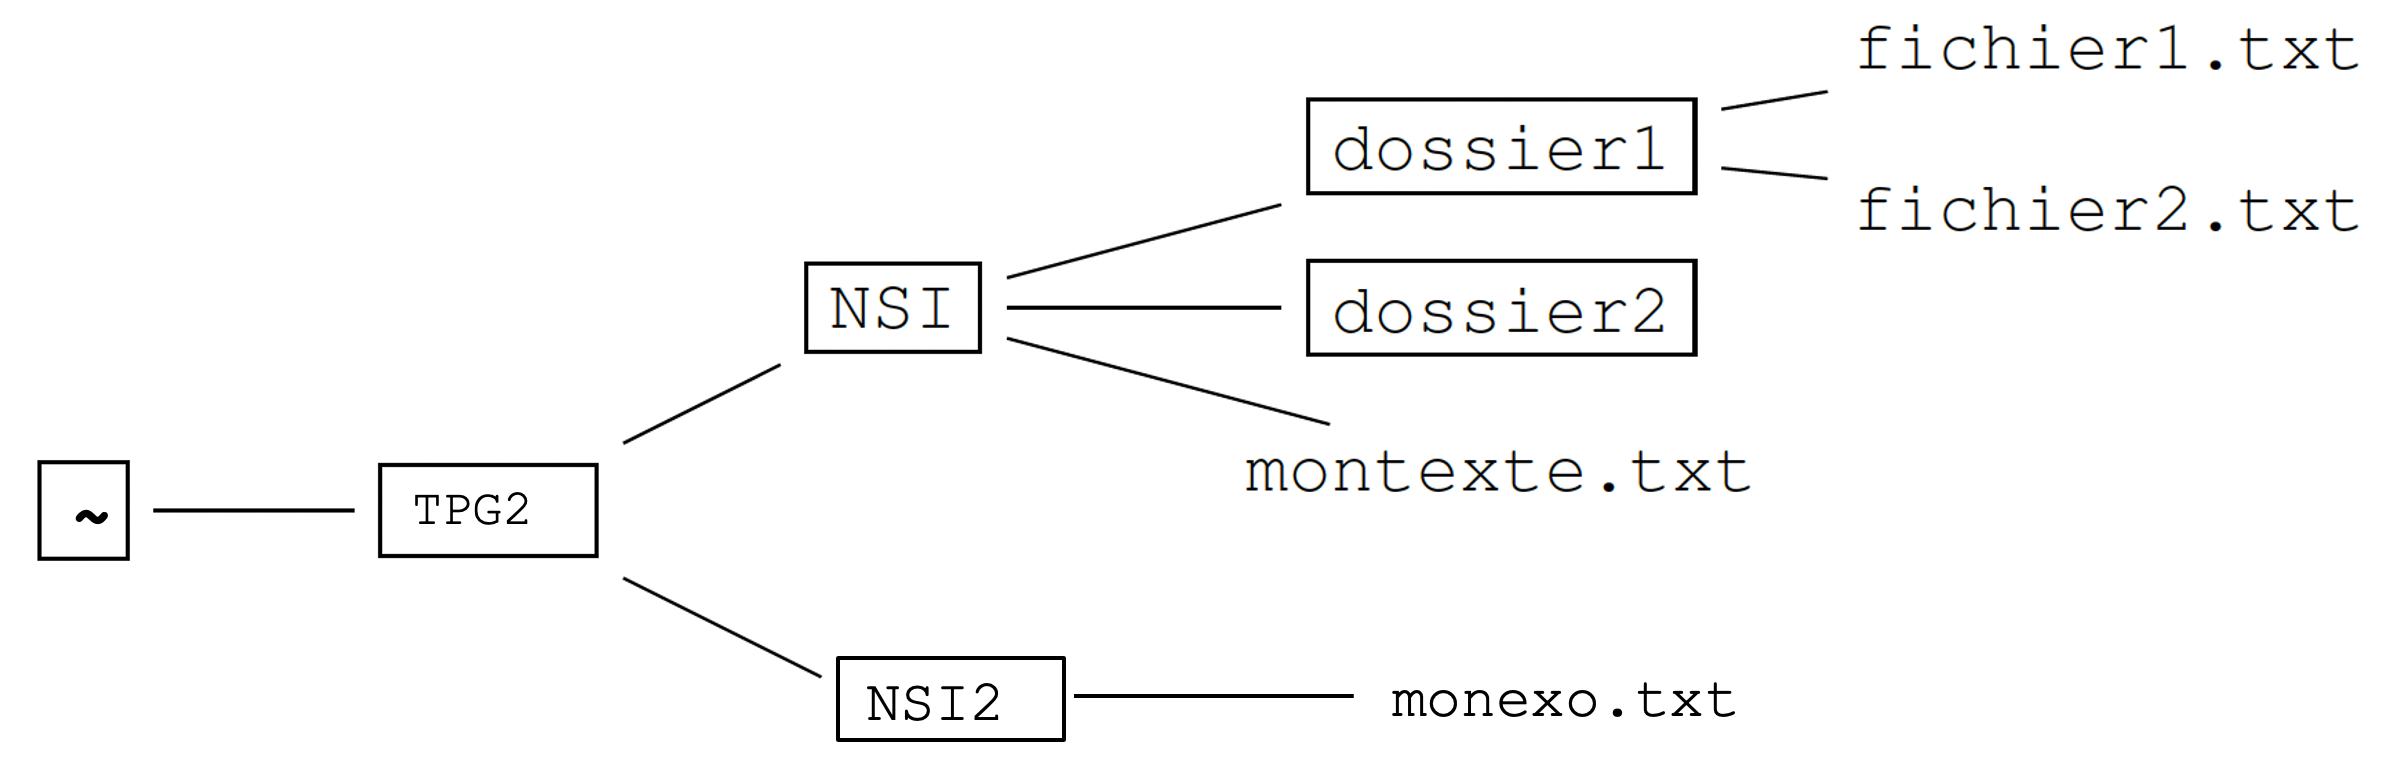
\includegraphics[width=0.9\textwidth]{013_TP_Arbo.png}
	\end{figure}
	
	\begin{itemize}
		\item Le répertoire de base dans cette représentation est le répertoire personnel de l'utilisateur de l'ordinateur que par convention on note "$\sim$". Sur vos machines il s'agit du répertoire \texttt{/home/nsi} et c'est là que s'ouvre votre terminal .
		\item Dans cet exemple il y a un répertoire dans $\sim$: \texttt{TPG2}.
		\item Dans cet exemple il y a deux répertoires dans $\sim$\texttt{/TPG2}, \texttt{NSI} et \texttt{NSI2}.
		\item Le fichier \texttt{montexte.txt} est directement dans le répertoire \texttt{NSI}.
		\item Le fichier \texttt{fichier2.txt} est dans le répertoire \texttt{dossier1} qui est un sous-répertoire de \texttt{NSI}.
		\item Etc...
	\end{itemize}
	
	Voici un certain nombre de commandes utiles pour naviguer dans l'arborescence de fichiers et créer de nouveaux répertoires et fichiers:
	
	\begin{figure}[H]
		\centering
		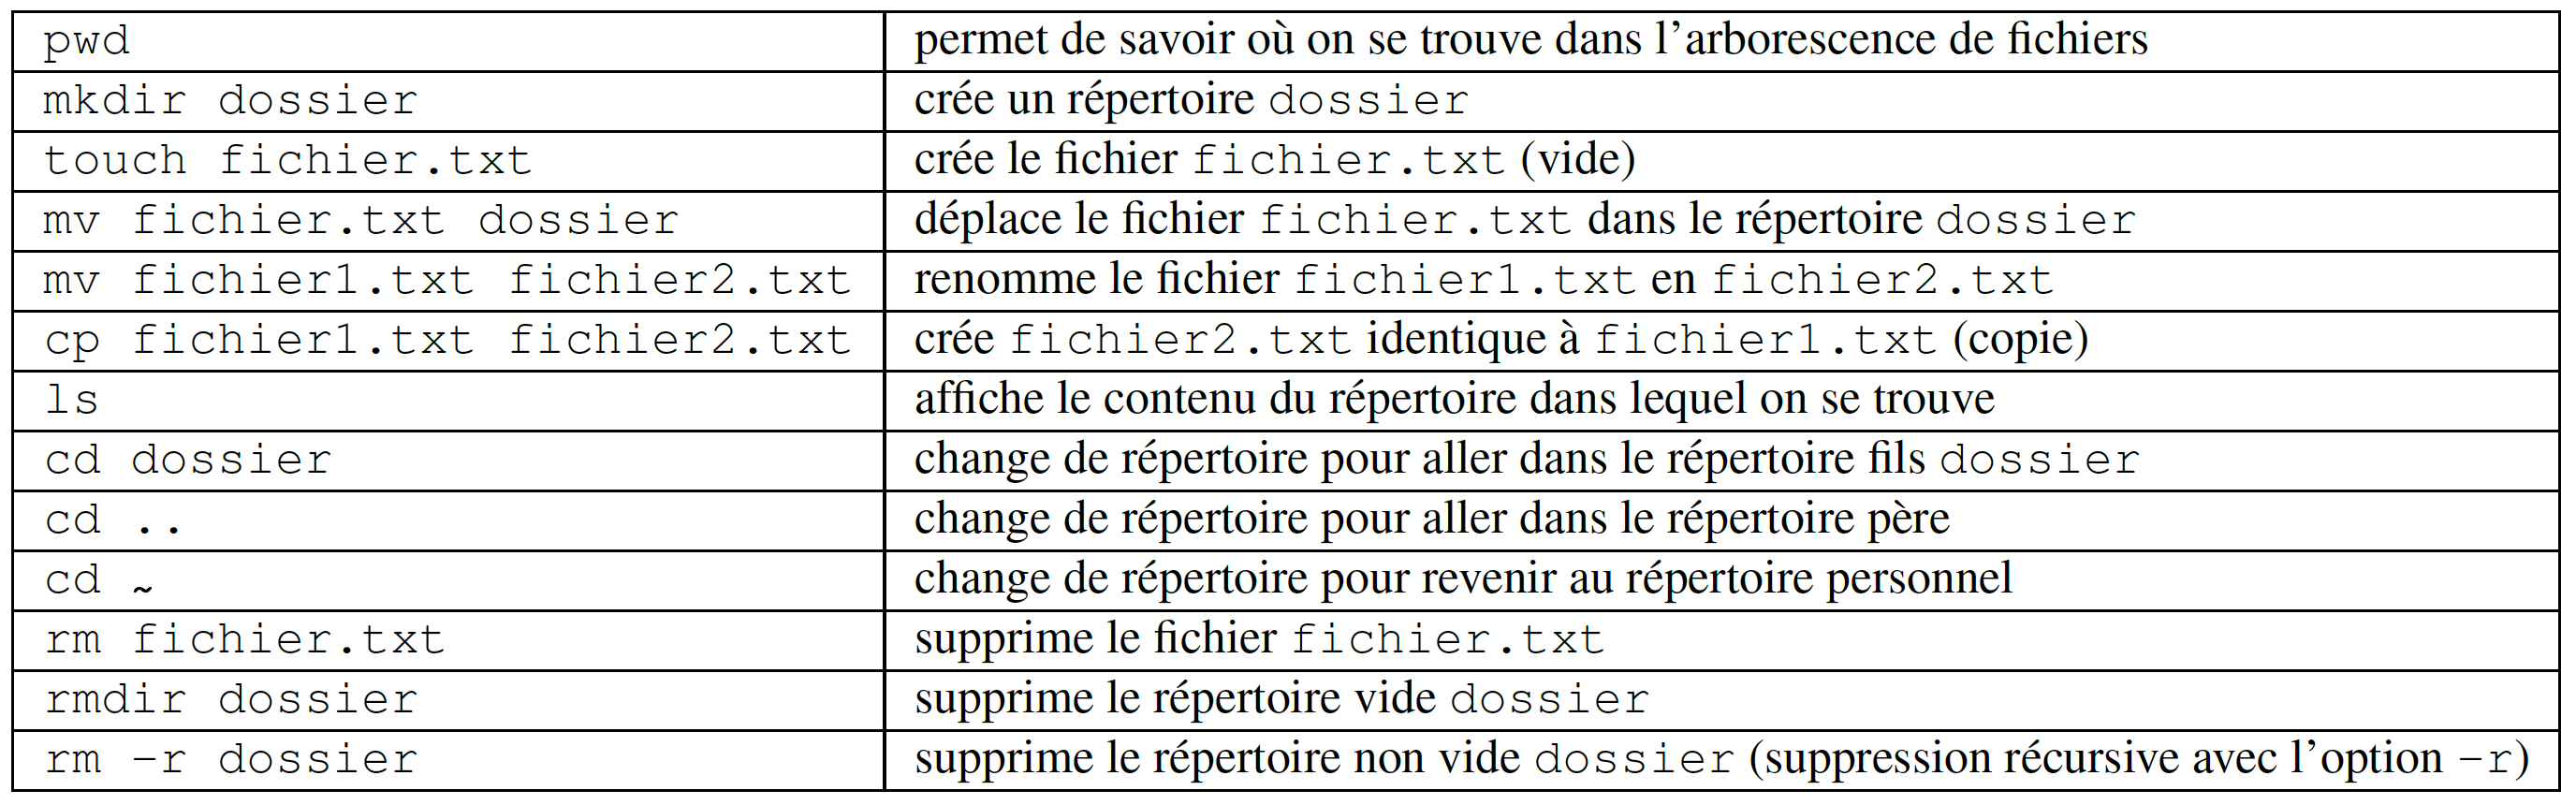
\includegraphics[width=\textwidth]{014_TP_Cmds.png}
	\end{figure}
	
	\begin{MonExo}[Manipulations élémentaires de fichiers]
		\begin{alphenum}
			\item Assurez-vous d'abord de bien être dans le répertoire personnel de votre utilisateur: tapez \texttt{pwd}, puis \textit{Entrée}: obtenez-vous bien \texttt{/home/nsi}?
			\item A l'aide des commandes ci-dessus, reproduisez l'arborescence du schéma plus haut (\texttt{TPG2} etc...).
			\item Enrichissez votre arborescence:
			\begin{enumerate}
				\item Créez dans \texttt{NSI2} deux répertoires: \texttt{essai1} et \texttt{essai2}.
				\item Créez dans \texttt{essai2} un fichier \texttt{text.txt}.
				\item Dupliquez ce fichier dans le même répertoire en deux fichiers \texttt{text1.txt} et \texttt{text2.txt}.
				\item Déplacez \texttt{text1.txt} dans le répertoire \texttt{dossier2} de l'arborescence.
				\item Déplacez-vous dans tous les répertoires pour vérifier que le contenu est le bon.
				\item En une seule commande supprimez toute la sous-arborescence \texttt{NSI2}.
			\end{enumerate}
		\end{alphenum}
	\end{MonExo}
	
	\section{Gérer l'administration des droits}
	
	La commande \texttt{ls} possède les options suivantes:
	\begin{figure}[H]
		\centering
		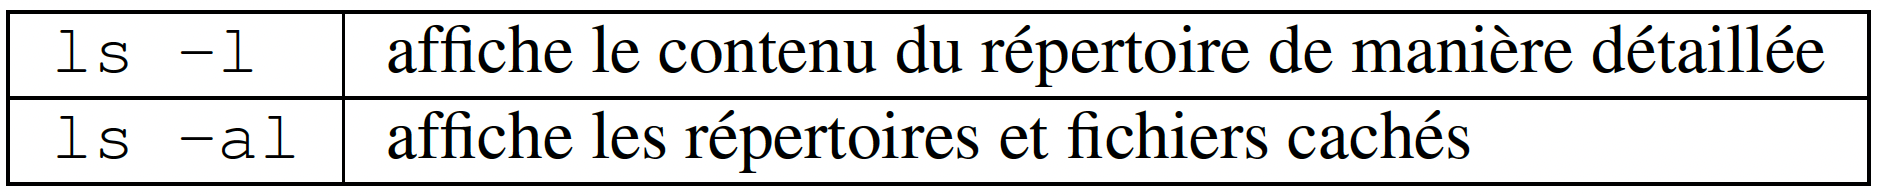
\includegraphics[width=0.6\textwidth]{015_TP_OptionsLs.png}
	\end{figure}
	
	Le rendu d'un \texttt{ls -l} pourrait ressembler à ceci:
	 \begin{figure}[H]
	 	\centering
	 	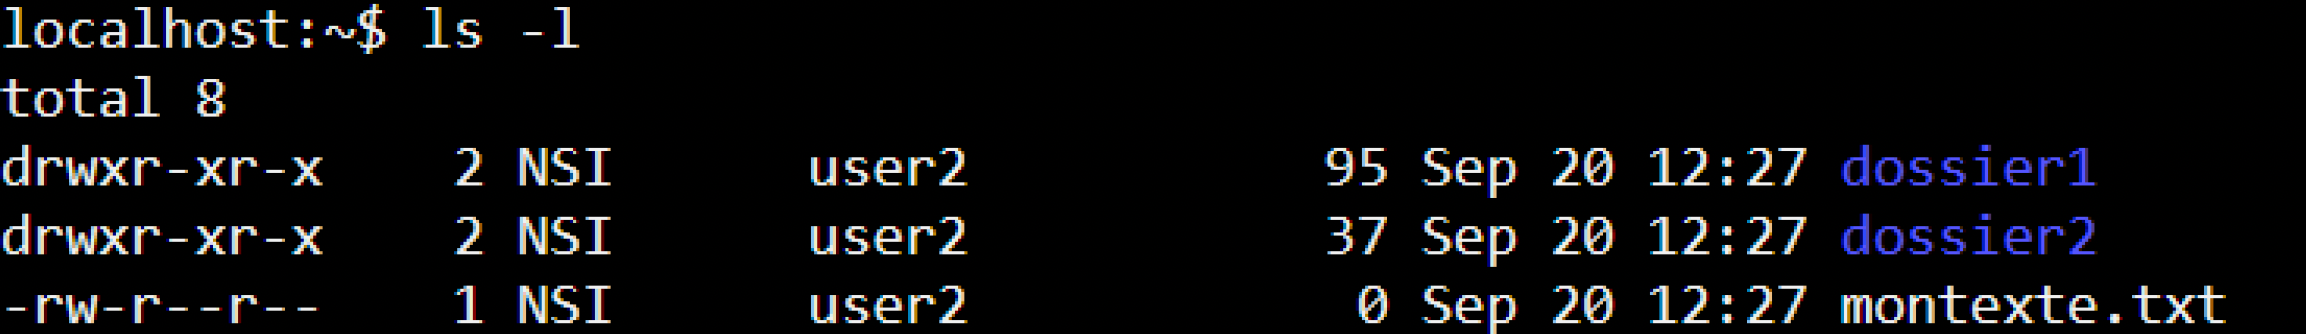
\includegraphics[width=0.8\textwidth]{016_TP_Ls-al.png}
	 \end{figure}
	 
	 Dans l'ordre, cela se lit, de gauche à droite:
	 
	 \textbf{droits - nombre de liens - nom du propriétaire - nom du groupe - taille en octet - date - heure - nom du fichier ou du répertoire}

	Les systèmes de type \texttt{UNIX} sont des systèmes multi-utilisateurs. Plusieurs utilisateurs peuvent donc partager un même ordinateur. Comme chaque utilisateur possède un environnement de travail qui lui est propre (avec pour répertoire personnel \texttt{/home/nsi} dans notre cas ici), chaque utilisateur possède certains droits lui permettant d'effectuer certaines opérations et pas d'autres. On peut gérer ces droits par le shell.
	
	Il faut distinguer un utilisateur un peu particulier qui est autorisé à modifier tous les droits: ce "super utilisateur" est appelé "administrateur" ou "root".
	
	Au lieu de gérer les utilisateurs un par un, il est possible de créer des groupes d'utilisateurs. L'administrateur peut alors attribuer des droits à un groupe directement. Remarque: dans l'exemple donné ci-dessus, le nom du groupe est \texttt{user2} et celui du propriétaire \texttt{NSI}.
	
	Ainsi les fichiers et les répertoires possèdent 3 types de droits:
	\begin{itemize}
		\item Les droits en lecture: \texttt{r} (Read) signifie que la lecture est autorisée;
		\item Les droits en écriture: \texttt{w} (Write) signifie que l'écriture est autorisée;
		\item Les droits en exécution: \texttt{x} (eXecute) signifie que l'exécution est autorisée.
		\item Un tiret "\texttt{-}" interdit le droit en question.
		\item Les droits sont listés d'abord pour le propriétaire du fichier, puis pour les membres de son groupe, puis pour tous les autres utilisateurs.
	\end{itemize}
	
	Ainsi, pour le fichier \texttt{montexte.txt} dans l'exemple précédent, dont les droits sont écrits "\texttt{-rw-r-\,-r-\,-}", les droits sont:
	\begin{itemize}
		\item Le premier caractère, "\texttt{-}" indique que c'est un fichier et non un répertoire (on aurait alors \texttt{d} comme Directory);
		\item \texttt{rw-} pour le propriétaire: accès en lecture et en écriture;
		\item \texttt{r-\,-} pour le groupe et tous les autres: accès en lecture seulement;
		\item On n'a pas évidemment de \texttt{x} ici puisque l'exécution d'un fichier texte n'a pas de sens.
	\end{itemize}
	
	Pour changer les droits d'un fichier ou dossier, on utilise la commande \texttt{chmod} suivie d'un nombre composé de 3 chiffres (un pour le propriétaire, un pour le groupe, un pour les autres) puis du nom du fichier concerné. Pour savoir quel nombre on choisit il suffit de savoir compter en binaire. Par exemple:
	\begin{itemize}
		\item \texttt{rwx} correspondra au nombre binaire 111 donc au nombre entier 7;
		\item \texttt{rw-} correspondra au nombre binaire 110 donc au nombre entier 6;
		\item \texttt{r-\,-} correspondra au nombre binaire 100 donc au nombre entier 4.
	\end{itemize}
	
	Donc par exemple si l'on voulait modifier les droits de \texttt{montexte.txt} pour donner le droit en écriture au groupe mais sans le donner à tout le monde on taperait la commande: \texttt{chmod 664 montexte.txt} (6 pour le propriétaire et le groupe, 4 pour les autres).
	
	\begin{MonExo}[Gestion des droits d'un fichier]
		\begin{alphenum}
			\item Quel nombre de 3 chiffres doit-on choisir pour qu'un fichier soit accessible en lecture uniquement au propriétaire et au groupe, accessible en exécution à tous et uniquement accessible en écriture au propriétaire? Testez votre commande sur le fichier \texttt{montexte.txt}
			\item Changez les droits du répertoire dossier2 en \texttt{rwxrw-r-\,-}
			\item Tapez la commande \texttt{chown --help}. A quoi sert la commande chown?
		\end{alphenum}
	\end{MonExo}
	
	\pagebreak
	\section{Travail à rendre sur papier}
	
	Rien de ce qui précède n'est à rendre --- mais si tout a été fait, cet exercice, à rendre sur papier, devrait être extrêmement simple et rapide à effectuer.
	
	\begin{MonExo}[A rendre]
		On considère l'arborescence suivante:
		
		\begin{figure}[H]
			\centering
			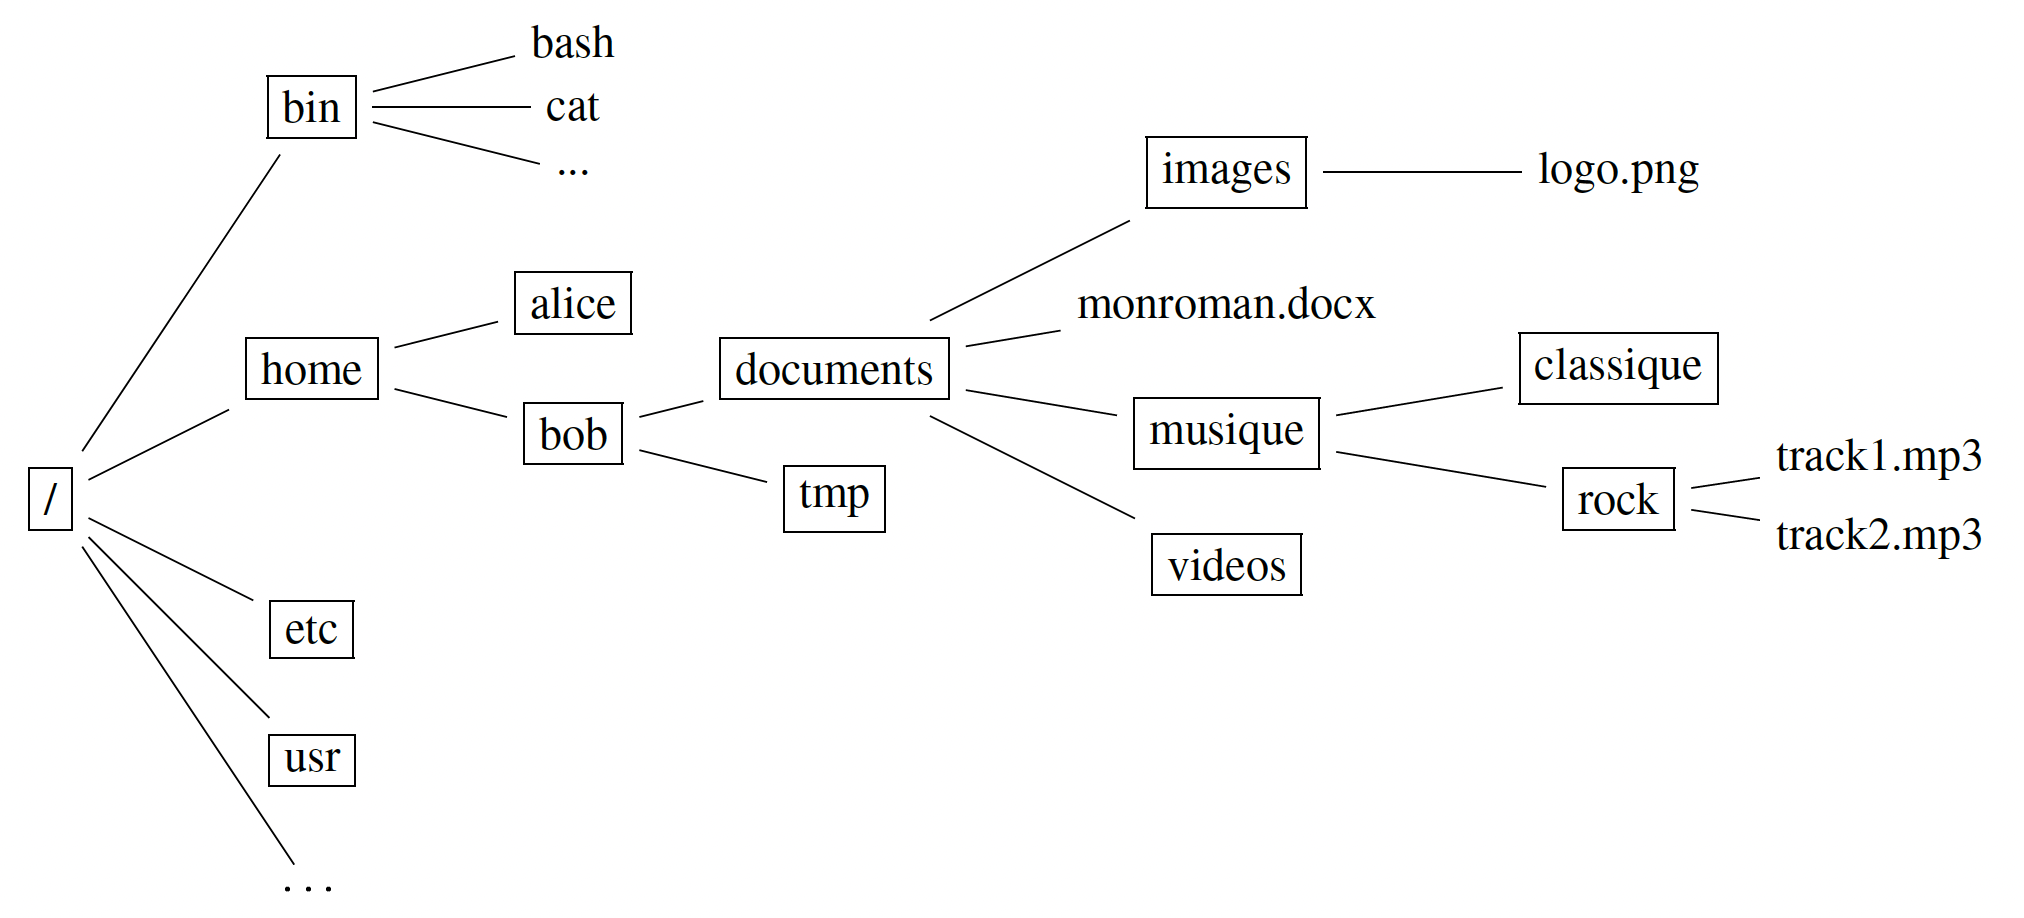
\includegraphics[width=0.9\textwidth]{017_TP_ArboExo.png}
		\end{figure}
		\begin{alphenum}
			\item En supposant que je me trouve dans le dossier \texttt{documents}, que sera-t-il affiché dans la console si je tape \texttt{pwd}?
			\item En supposant que je me trouve dans le dossier \texttt{images}, quelle commande dois-je-saisir si je veux aller dans le dossier \texttt{musique}?
			\item Quelle est la différence entre les commandes \text{cp test1.txt text2.txt} et \text{mv test1.txt text2.txt}?
			\item Si je saisis la commande \texttt{rm videos} à partir du dossier \texttt{documents} que se passe-t-il?
			\item Si je veux détruire le dossier \texttt{rock} quelle commande dois-je saisir?
			\item Pour connaître les droits du fichier \texttt{monroman.docx} que faut-il saisir ?
			\item Si je veux changer les droits de \texttt{monroman.docx} afin d'être la seule personne à pouvoir le lire et le modifier, que dois-je saisir
dans le shell ? On supposera également que personne ne pourra exécuter ce fichier.
		\end{alphenum}
	\end{MonExo}
	
	\section{Défi -- pour ceux qui le souhaitent}
	\begin{MonExo}[Quelques défis pour aller plus loin]
		\begin{alphenum}
			\item Automatiser la création de 100 répertoires nommés \texttt{rep1} à \texttt{rep100} dans le répertoire \texttt{dossier2}.
			\item Copier tous les fichiers \texttt{.txt} du répertoire \texttt{dossier1} vers \texttt{dossier2} uniquement si leur taille dépasse 1KB.
			\item Supprimer tous les fichiers temporaires (extension \texttt{.tmp}) dans \texttt{/home/nsi} qui ont été modifiés il y a plus de 7 jours.
		\end{alphenum}
	\end{MonExo}
\end{document}
